\documentclass[tikz,border=7pt]{standalone}
% Shared TikZ style for the Nios V stereo accelerator diagrams.
\usepackage[T1]{fontenc}
\usepackage{lmodern}
\usepackage{xcolor}
\usepackage{tikz}
\usetikzlibrary{arrows.meta,backgrounds,calc,fit,positioning}

\definecolor{navy}{HTML}{073D73}
\definecolor{blue}{HTML}{0B5CAB}
\definecolor{cyan}{HTML}{1B8DBB}
\definecolor{green}{HTML}{27845B}
\definecolor{orange}{HTML}{C66A16}
\definecolor{red}{HTML}{B94444}
\definecolor{ink}{HTML}{172033}
\definecolor{muted}{HTML}{5A6678}
\definecolor{line}{HTML}{BFCBDA}
\definecolor{softblue}{HTML}{EDF4FA}
\definecolor{softcyan}{HTML}{ECF8FB}
\definecolor{softgreen}{HTML}{EEF8F2}
\definecolor{softorange}{HTML}{FFF4E8}
\definecolor{softgray}{HTML}{F5F7FA}

% Avoid automatic word hyphenation inside compact diagram nodes.
\hyphenpenalty=10000
\exhyphenpenalty=10000

\tikzset{
  font=\sffamily,
  block/.style={
    draw=line, rounded corners=2.2pt, fill=white,
    minimum height=10mm, text width=31mm, align=center,
    inner xsep=3mm, inner ysep=2.2mm
  },
  cpu/.style={block, draw=blue!55, fill=softblue},
  accel/.style={block, draw=cyan!65, fill=softcyan},
  memory/.style={block, draw=green!60, fill=softgreen},
  control/.style={block, draw=orange!65, fill=softorange},
  smallblock/.style={block, text width=24mm, minimum height=8mm, inner xsep=2mm, inner ysep=1.6mm},
  group/.style={draw=line, rounded corners=4pt, fill=softgray, inner sep=4mm},
  labeltag/.style={rounded corners=2pt, fill=navy, text=white, font=\sffamily\bfseries\footnotesize, inner xsep=2.5mm, inner ysep=1.2mm},
  flow/.style={-{Stealth[length=2.6mm,width=1.8mm]}, draw=navy, line width=0.85pt},
  dataflow/.style={-{Stealth[length=2.8mm,width=2mm]}, draw=blue, line width=1.15pt},
  controlflow/.style={-{Stealth[length=2.4mm,width=1.7mm]}, draw=orange, line width=0.9pt, dashed},
  returnflow/.style={-{Stealth[length=2.4mm,width=1.7mm]}, draw=green, line width=0.9pt},
  bus/.style={<->, >={Stealth[length=2.8mm,width=2mm]}, draw=navy, line width=1.6pt},
  note/.style={font=\sffamily\footnotesize, text=muted, align=left},
  arrowlabel/.style={font=\sffamily\scriptsize, text=muted, fill=white, inner sep=1.2pt}
}


\begin{document}
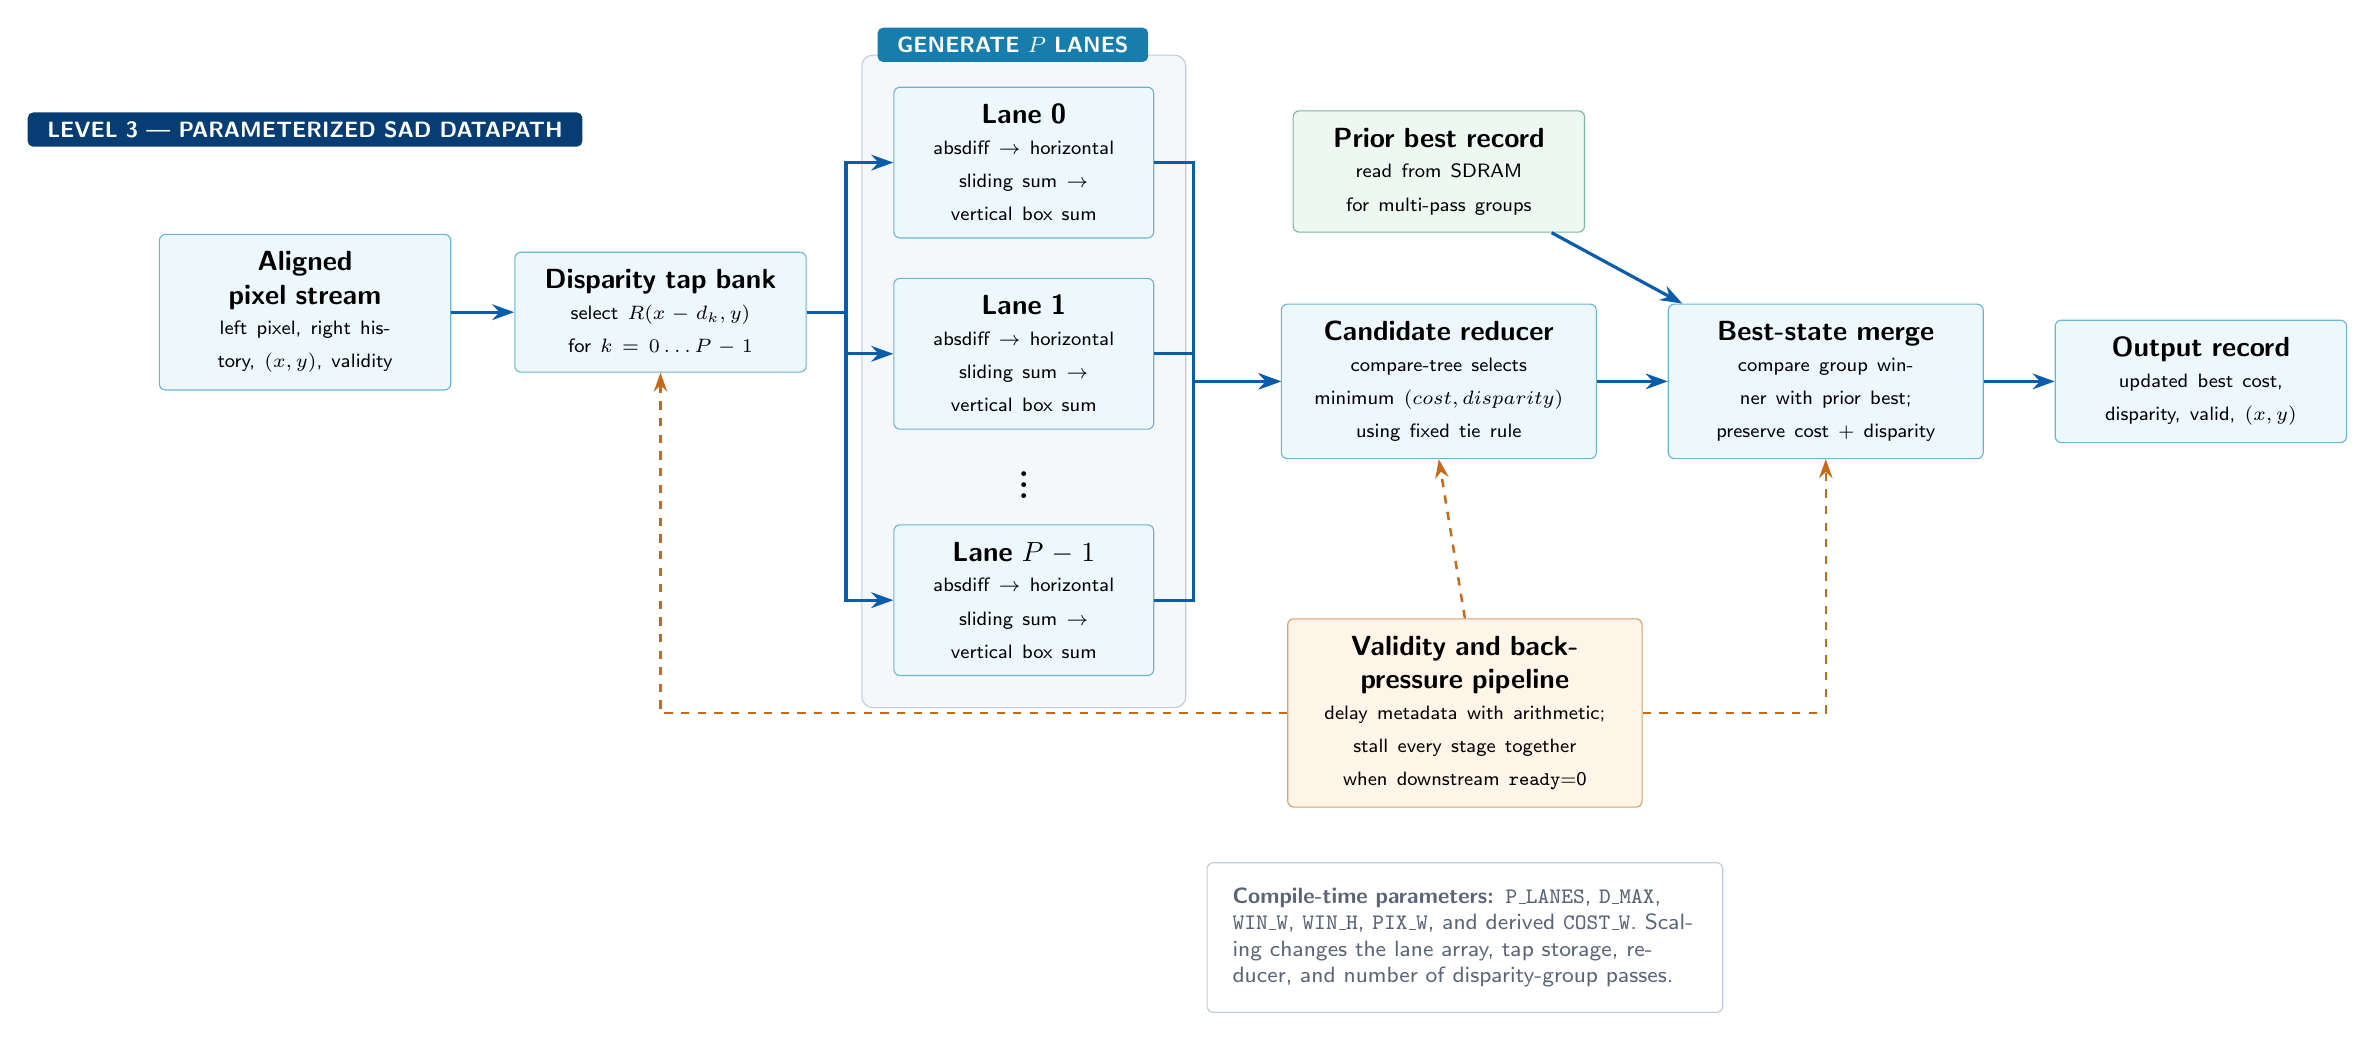
\begin{tikzpicture}[node distance=8mm and 8mm]
  \node[labeltag] (title) {LEVEL 3 --- PARAMETERIZED SAD DATAPATH};

  \node[accel, text width=31mm, below=11mm of title] (pixels) {\textbf{Aligned pixel stream}\\[-1pt]\scriptsize left pixel, right history, $(x,y)$, validity};
  \node[accel, text width=31mm, right=8mm of pixels] (taps) {\textbf{Disparity tap bank}\\[-1pt]\scriptsize select $R(x-d_k,y)$ for $k=0\ldots P-1$};

  \node[accel, text width=27mm, right=11mm of taps, yshift=19mm] (lane0) {\textbf{Lane 0}\\[-1pt]\scriptsize absdiff $\rightarrow$ horizontal sliding sum $\rightarrow$ vertical box sum};
  \node[accel, text width=27mm, below=5mm of lane0] (lane1) {\textbf{Lane 1}\\[-1pt]\scriptsize absdiff $\rightarrow$ horizontal sliding sum $\rightarrow$ vertical box sum};
  \node[font=\bfseries\large, below=2mm of lane1] (dots) {$\vdots$};
  \node[accel, text width=27mm, below=2mm of dots] (lanep) {\textbf{Lane $P-1$}\\[-1pt]\scriptsize absdiff $\rightarrow$ horizontal sliding sum $\rightarrow$ vertical box sum};
  \begin{scope}[on background layer]
    \node[group, fit=(lane0)(lane1)(dots)(lanep)] (lanes) {};
  \end{scope}
  \node[labeltag, anchor=south west, fill=cyan!80!navy] at ([xshift=2mm,yshift=-1mm]lanes.north west) {GENERATE $P$ LANES};

  \node[accel, text width=34mm, right=12mm of lanes] (reduce) {\textbf{Candidate reducer}\\[-1pt]\scriptsize compare-tree selects minimum $(cost, disparity)$ using fixed tie rule};
  \node[memory, text width=31mm, above=9mm of reduce] (prior) {\textbf{Prior best record}\\[-1pt]\scriptsize read from SDRAM for multi-pass groups};
  \node[accel, text width=34mm, right=9mm of reduce] (merge) {\textbf{Best-state merge}\\[-1pt]\scriptsize compare group winner with prior best; preserve cost + disparity};
  \node[accel, text width=31mm, right=9mm of merge] (out) {\textbf{Output record}\\[-1pt]\scriptsize updated best cost, disparity, valid, $(x,y)$};

  \draw[dataflow] (pixels) -- (taps);
  \draw[dataflow] (taps.east) -- ++(5mm,0) |- (lane0.west);
  \draw[dataflow] (taps.east) -- ++(5mm,0) |- (lane1.west);
  \draw[dataflow] (taps.east) -- ++(5mm,0) |- (lanep.west);
  \draw[dataflow] (lane0.east) -- ++(5mm,0) |- (reduce.west);
  \draw[dataflow] (lane1.east) -- ++(5mm,0) |- (reduce.west);
  \draw[dataflow] (lanep.east) -- ++(5mm,0) |- (reduce.west);
  \draw[dataflow] (reduce) -- (merge);
  \draw[dataflow] (prior) -- (merge);
  \draw[dataflow] (merge) -- (out);

  \node[control, text width=39mm] (valid) at ($(lanes.south)!0.55!(merge.south)+(0,-18mm)$) {\textbf{Validity and backpressure pipeline}\\[-1pt]\scriptsize delay metadata with arithmetic; stall every stage together when downstream \texttt{ready}=0};
  \draw[controlflow] (valid.north) -- (reduce.south);
  \draw[controlflow] (valid.west) -| (taps.south);
  \draw[controlflow] (valid.east) -| (merge.south);

  \node[note, text width=59mm, below=9mm of valid] (params) {\textbf{Compile-time parameters:} \texttt{P\_LANES}, \texttt{D\_MAX}, \texttt{WIN\_W}, \texttt{WIN\_H}, \texttt{PIX\_W}, and derived \texttt{COST\_W}. Scaling changes the lane array, tap storage, reducer, and number of disparity-group passes.};
  \draw[draw=line, rounded corners=2pt] ([xshift=-2mm,yshift=-2mm]params.south west) rectangle ([xshift=2mm,yshift=2mm]params.north east);
\end{tikzpicture}
\end{document}
